% !Mode:: "TeX:UTF-8"

\chapter{姿态估计相关理论基础}

\section{引言}

人体姿态估计是人机交互的基础,学者们做了很多工作。从基于传感器的模型,到基于图模型的研究,再到如今基于深度学习方法的流行,其热度始终不减。但依旧无法满足应用场景。从绪论我们可以看出,当今人体姿态估计算法的方向是轻量化,快速化,准确化。

本章节主要介绍一些比较基础但十分重要的深度学习概念,为下面BlazePose算法的诞生做铺垫。首先我们会介绍卷积神经网络的各个组成部件,其次会深入了解反向传播算法,然后介绍常见的激活函数,最后为抑制过拟合现象介绍一些正则化方法。

\section{卷积神经网络的组成}

一个基本的卷积神经网络是由多个卷积层与池化层组成的卷积块以及全连接层相互连接而成。如图~\ref{piture:4}~所示。由$M(2\leqslant M\leqslant 5)$个连续的卷积层和$b(b\text{取}0\text{或}1)$个池化层组成一个卷积模块。再由$N$个连续的卷积模块和$K(0\leqslant K\leqslant 2)$个全连接层堆叠而成。

\begin{figure}[h]
\centering
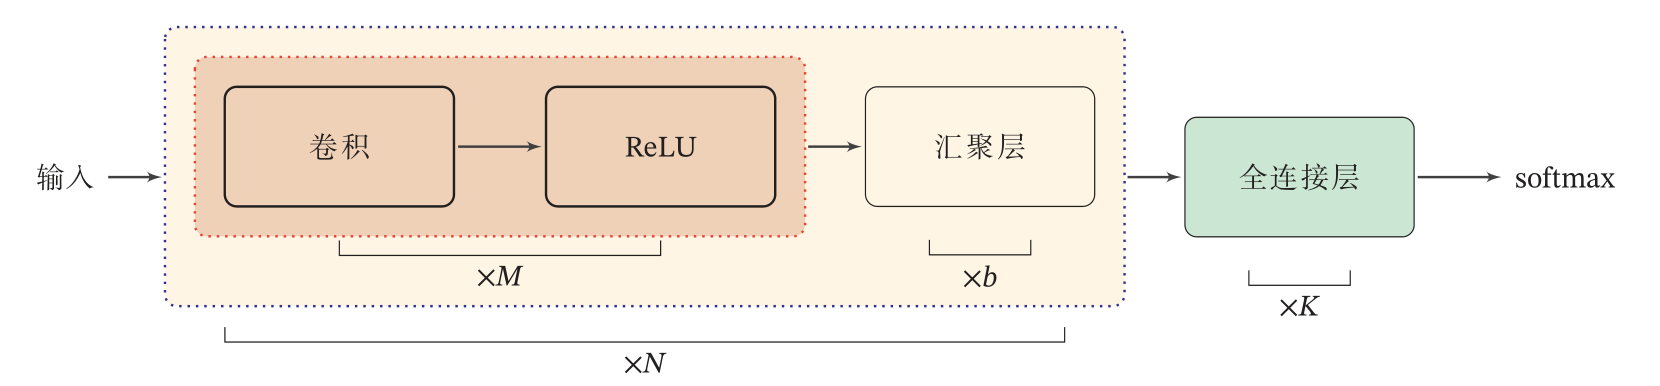
\includegraphics[width = 1\textwidth]{net}
\caption{常用卷积网络整体结构}
\label{piture:4}
\end{figure}

\subsection{卷积层}
卷积层的作用是提取特征,浅层网络可以提取到边缘,颜色等浅层信息;深层网络可以提取到形状,图案等深层的语义信息。其中,使用不同的滤波器即卷积核,提取到的信息也不尽相同。不失一般性,我们假设卷积神经网络处理的是二维图像,那么我们将通常使用三维的、大小是$M\times N\times D$神经层,其中$M,N,D$分别为高度,宽度,深度。

由此可以假设卷积层的结构如下:

\begin{enumerate}
\item 由三维张量$x\in \mathbb{R}^{M\times N\times D}$组成的输入特征映射组,其中$1\leqslant d\leqslant D$;

\item 由三维张量$y\in \mathbb{R}^{M'\times N'\times P}$组成的输出特征映射组,其中$1\leqslant p\leqslant P$;

\item 由四维张量$w\in \mathbb{R}^{U\times V\times P\times D}$组成的卷积核,其中$1\leqslant p\leqslant P,1\leqslant d\leqslant D$。
\end{enumerate}

卷积层的三维结构表示如图~\ref{piture:5}~所示。

\begin{figure}[h]
\centering
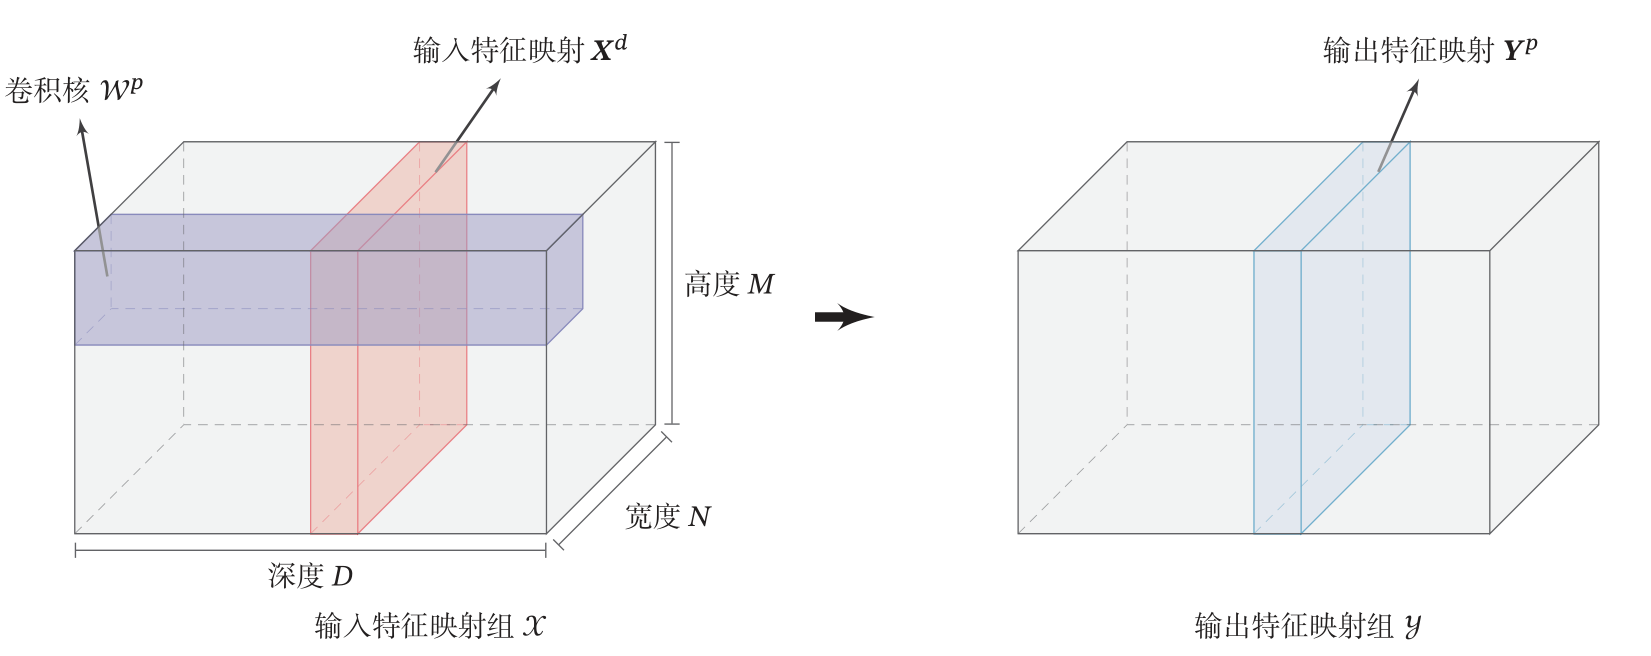
\includegraphics[width = 1\textwidth]{3-d}
\caption{卷积层的三维结构表示}
\label{piture:5}
\end{figure}

将卷积核$W^{p,1},W^{p,2},\cdots,W^{p,D}$和输入特征映射$X^1,X^2,\cdots,X^D$一一对应分别进行卷积操作,并与偏置量$b$求和。可以得到卷积层输出$Z^p$,最后再经过激活函数的激活,即可得到输出特征映射$Y^{p}$。

\begin{equation}
\label{eq:2}
\begin{aligned}
Z^p&=W^p\otimes X+b^p=\sum_{d=1}^{D}W^{p,d}\otimes X^d+b^p\\
Y^p&=f(Z^p)
\end{aligned}
\end{equation}

值得注意的是,对于激活函数$f(\cdot)$,我们一般使用ReLU函数。

计算过程的流程图如图~\ref{piture:6}~所示。

\begin{figure}[h]
\centering
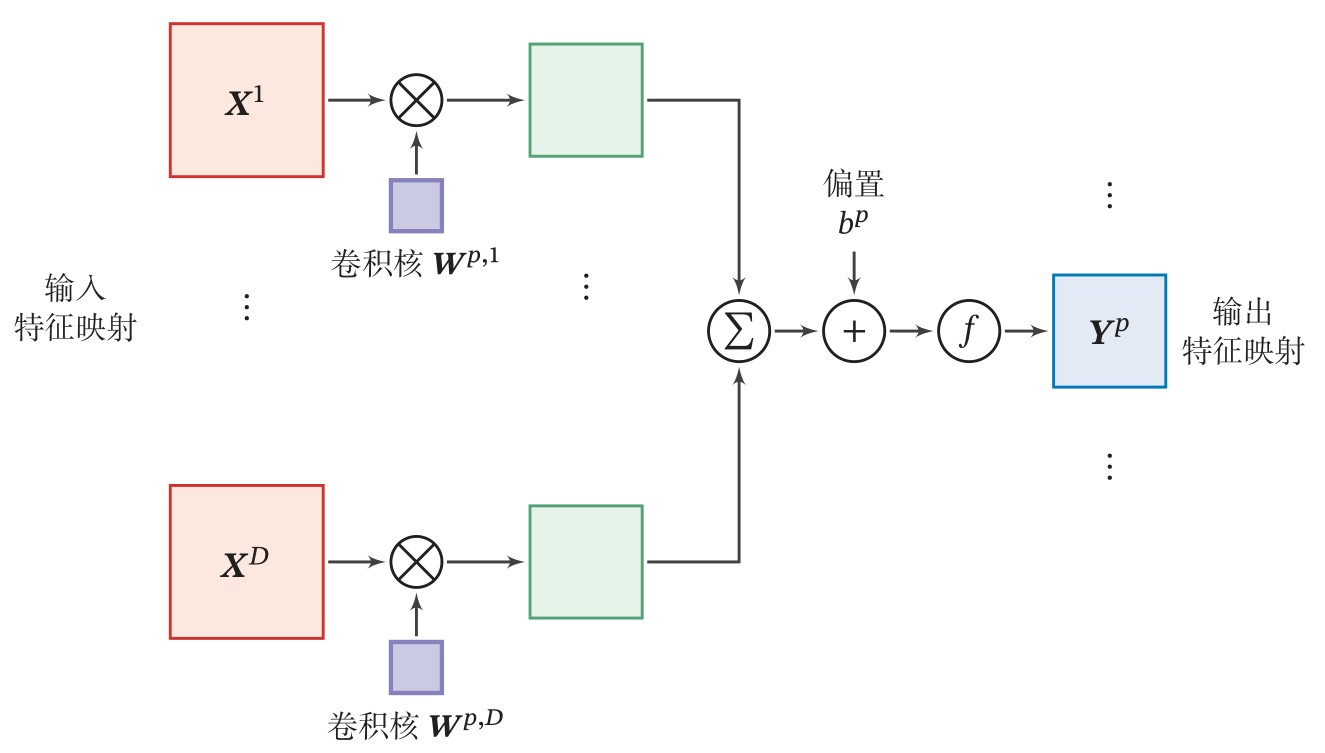
\includegraphics[width = 0.6\textwidth]{count}
\caption{卷积层中的计算流程图}
\label{piture:6}
\end{figure}

\subsection{池化层}

池化层通俗地说,池化就是将矩阵的各个子矩阵压缩。例如,如果我们想对一个$4\times 4$的矩阵进行$2\times 2$的池化,那么就会将$4\times 4$的矩阵拆分成$4$个$2\times 2$的子矩阵。并将每个子矩阵经过池化变成一个标量。一般而言,池化标准可以是最大池化,也可以是平均池化。对于前者,在每个子矩阵的元素中取出一个最大的作为结果;对于后者,则是将子矩阵的各个元素的平均值作为结果。从而达到降维的效果。

接下来,我们举一个采用$2\times 2$最大池化,步幅为$2$的例子。如图~\ref{piture:6}~所示。

首先,我们以一个$4\times 4$的输入矩阵为例,将其拆分成$4$个$2\times 2$的子矩阵。对左上角的红色子矩阵使用最大池化,得到池化结果是该区域的最大值$6$。以此类推,右上角的绿色矩阵结果为$8$,左下角的黄色区域池化结果为$3$,右下角的蓝色区域结果为$4$。最终我们得到了一个$2\times 2$的矩阵,即池化的最终结果。可以看出,池化可以在保留一定的原信息的同时有效地降低矩阵维数,简化后续计算。


\begin{figure}[h]
\centering
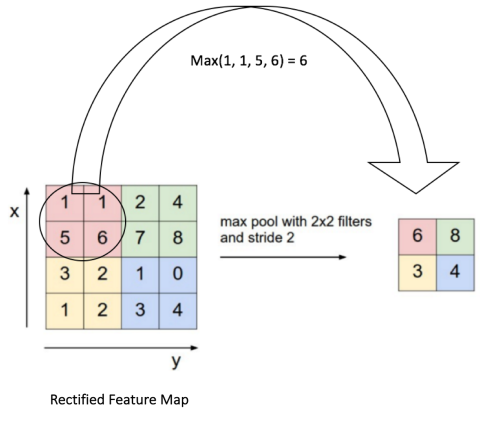
\includegraphics[width = 0.7\textwidth]{pool}
\caption{卷积层中从输入特征映射组$X$到输出特征映射$Y^p$的计算示例}
\label{piture:7}
\end{figure}

\section{卷积神经网络(CNN)反向传播算法}

\subsection{DNN的反向传播算法}

要计算DNN的反向传播,我们首先得出输出层的$\delta^L$

\begin{equation}
\label{eq:3}
\delta^L = \frac{\partial J(W,b)}{\partial z^L} = \frac{\partial J(W,b)}{\partial a^L}\odot \sigma^{'}(z^L)
\end{equation}

此外,使用第一数学归纳法,可以由$\delta^{l+1}$的值算出$\delta^l$如下:

\begin{equation}
\label{eq:4}
\delta^{l} = \delta^{l+1}\frac{\partial z^{l+1}}{\partial z^{l}} = (W^{l+1})^T\delta^{l+1}\odot \sigma^{'}(z^l)
\end{equation}

最后,我们可以得到出$W,b$的梯度:

\begin{equation}
\label{eq:5}
\begin{aligned}
\frac{\partial J(W,b)}{\partial W^l} &= \frac{\partial J(W,b,x,y)}{\partial z^l} \frac{\partial z^l}{\partial W^l} = \delta^{l}(a^{l-1})^T\\
\frac{\partial J(W,b,x,y)}{\partial b^l} &= \frac{\partial J(W,b)}{\partial z^l} \frac{\partial z^l}{\partial b^l} = \delta^{l}
\end{aligned}
\end{equation}

简单介绍完DNN的反向传播算法的推到思路后,我们将公式套用到CNN中,但需要注意的是,CNN与DNN还是有些许不同,这导致了我们需要解决几个问题,才能正确地套用。

\subsection{CNN的反向传播算法思想}

鉴于DNN与CNN的区别,我们再研究CNN反向传播的时候遇到了如下几个关键问题:

\begin{enumerate}
\item 池化层没有激活函数,这导致了我们无法从池化结果反向传播到输出。对此我们可以令激活函数是$\sigma(z) = z$;

\item 与DNN不同的是,图像经过池化层的前向传播时,受到了压缩,在数据被压缩的情况下,如何反向推导$\delta^{l-1}$;

\item 与DNN还有一点不同的是,DNN全连接层的输出是矩阵乘法得到的,而CNN的卷积层是通过卷积得到当前层的输出;

\item DNN中没有卷积层的概念,所以在求$W$时,要考虑到于$W$使用的是卷积运算。
\end{enumerate}

可以看出,第一点很容易就给出答案,所以问题2,3,4是解决CNN反向传播的难点。由于篇幅限制,下面直接给出结论:

对于问题2,我们有

\begin{equation}
\label{eq:6}
\delta_k^{l-1} = \frac{\partial J(W,b)}{\partial a_k^{l-1}} \frac{\partial  a_k^{l-1}}{\partial z_k^{l-1}} = upsample(\delta_k^l) \odot \sigma^{'}(z_k^{l-1})
\end{equation}

对于问题3,我们有

\begin{equation}
\label{eq:7}
\left( \begin{array}{cccc} 0&0&0&0 \\ 0&\delta_{11}& \delta_{12}&0 \\ 0&\delta_{21}&\delta_{22}&0 \\ 0&0&0&0 \end{array} \right) * \left( \begin{array}{ccc} w_{22}&w_{21}\\ w_{12}&w_{11} \end{array} \right)  = \left( \begin{array}{ccc} \nabla a_{11}&\nabla a_{12}&\nabla a_{13} \\ \nabla a_{21}&\nabla a_{22}&\nabla a_{23}\\ \nabla a_{31}&\nabla a_{32}&\nabla a_{33} \end{array} \right)
\end{equation}

对于问题4,我们有

\begin{equation}
\label{eq:8}
\frac{\partial J(W,b)}{\partial W^{l}} = \frac{\partial J(W,b)}{\partial z^{l}}\frac{\partial z^{l}}{\partial W^{l}} = \delta^l * rot180( a^{l-1})= \sum\limits_{u,v}(\delta^l)_{u,v}
\end{equation}

如此我们便可以得到算法~\ref{algo1}~。

\begin{algorithm}
\caption{反向传播算法(批量梯度下降法)}
\label{algo1}
\KwIn{$m,L,K,F,P,S,k,\alpha,MAX,\epsilon$,它们分别是图片样本数,模型层数,卷积核大小,卷积核子矩阵维度,填充大小,步幅,池化区域大小,梯度迭代步长,最大迭代次数,停止迭代的阈值。}
\KwOut{CNN各输出层的$W,b$}%

将所有层的$W,b$初始化成随机值。

\For{iter=1 to MAX}
{
	\For{$i=1$ to $m$}
	{
		将CNN输入$a^1$设置为$x_i$对应的张量
		
		\For{$l=2$ to $L-1$}
			{
				分3种情况计算前向传播:
				
				如果当前是全连接层:则有$a^{i,l} = \sigma(z^{i,l}) = \sigma(W^la^{i,l-1} + b^{i,l})$
				
				如果当前是卷积层:则有$a^{i,l} = \sigma(z^{i,l}) = \sigma(W^l*a^{i,l-1} + b^{i,l})$
				
				如果当前是池化层:则有$a^{i,l}= pool(a^{i,l-1})$
			}
		对于第$L$层输出层:$a^{i,L}= softmax(z^{i,L}) = softmax(W^{i,L}a^{i,L-1} +b^{i,L})$,通过损失函数计算输出层的$\delta^{i,L}$
		
		\For{$l=L$ to $2$}
			{
				分3种情况计算反向传播:
						
				如果当前是全连接层:$\delta^{i,l} =  (W^{l+1})^T\delta^{i,l+1}\odot \sigma^{'}(z^{i,l})$
						
				如果当前是卷积层:$\delta^{i,l} = \delta^{i,l+1}*rot180(W^{l+1}) \odot  \sigma^{'}(z^{i,l})$
						
				如果当前是池化层:$\delta^{i,l} =  upsample(\delta^{i,l+1}) \odot \sigma^{'}(z^{i,l})$
			}
	}
	\For{$l=2$ to $L$}
	{
	    根据下面$2$种情况更新第$l$层的$W^l,b^l$:
	    
	    如果当前是全连接层:$W^l = W^l -\alpha \sum\limits_{i=1}^m \delta^{i,l}(a^{i, l-1})^T$$ $$b^l = b^l -\alpha \sum\limits_{i=1}^m \delta^{i,l}$
	    
	    如果当前是卷积层,对于每一个卷积核有:$W^l = W^l -\alpha \sum\limits_{i=1}^m \delta^{i,l}* rot180(a^{i, l-1}), b^l = b^l -\alpha \sum\limits_{i=1}^m \sum\limits_{u,v}(\delta^{i,l})_{u,v}$
	}
	若$W,b$的变化值不大于阈值$\epsilon$,跳出循环。
	
	输出各层的$W$和$b$,其中$W$是线性关系系数矩阵,$b$是偏倚向量。
}
\end{algorithm}

\section{激活函数}

本质上,卷积神经网络就是由多个感知机组成的,所以,如果没有其他操作,最后的结果肯定相当于一个线性变换,这使得神经网络处理信息的能力很弱。故而我们引入激活函数,来模拟人脑神经元突触的激活效果,从而使得卷积网络脱离线性关系,以获得更强的学习能力。这里我们主要介绍三种激活函数:Sigmoid,tanh,ReLU。

\subsection{Sigmoid激活函数}

sigmoid函数及其导数如图~\ref{piture:8}~所示。

从sigmoid函数的导数我们可以看出,它可以用sigmoid函数自身来表示,所以梯度计算较为方便。此外它的梯度也比较平滑,它将一个$(-\infty ,+\infty)$之内的实数值变换到区间$[0,1]$之间,还满足处处连续。但是它也有着很严重的缺点:一方面,求导计算量大,反向传播过程中计算loss值的梯度时还会涉及除法;另一方面,由于当输入值在[-4,4]之间时导数值比较大,其余部分导数值趋于0,很容易出现梯度消失的情况,从而无法实现深层网络的训练。

\begin{figure}[h]
\centering
\includegraphics[width = 1\textwidth]{sigmoid}
\caption{sigmoid函数及其导数}
\label{piture:8}
\end{figure}

\subsection{tanh激活函数}

tanh函数及其导数如图~\ref{piture:9}~所示。

与sigmoid函数不同的是,tanh函数将输出域从$(0,1)$改到$(-1,1)$,让输出以$0$为中心,有便于神经网络归一化特征的学习。此外,tanh函数的梯度消失问题比sigmoid要轻,收敛更快。但是,当输入太大或者太小的时候,tanh函数的值无限接近$-1$或者$1$,此时的梯度为$0$,梯度消失问题依旧很严重。

\begin{figure}[h]
\centering
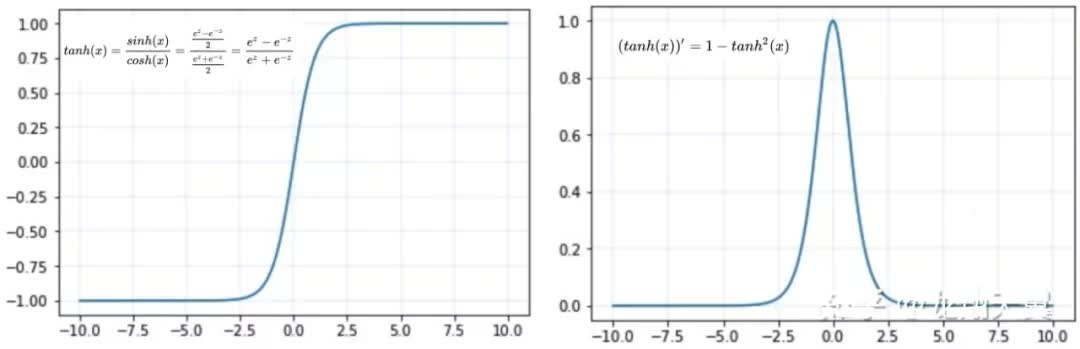
\includegraphics[width = 1\textwidth]{tanh}
\caption{tanh函数及其导数}
\label{piture:9}
\end{figure}

\subsection{整流线性单元(ReLU)}

ReLU函数及其导数如图~\ref{piture:10}~所示。

为了缓解梯度消失问题,ReLU函数被提出来。它简单高效,不涉及指数等运算;而且ReLU激活函数的导数在变动很大的情况下,会远大于于$0$;此外,ReLu激活函数会使神经网络学习效率变高;最后,当$x>0$时,ReLU函数的导数是常数,这有效地解决了梯度弥散现象。这些使得它成为当今最主流的激活函数之一。

\begin{figure}[h]
\centering
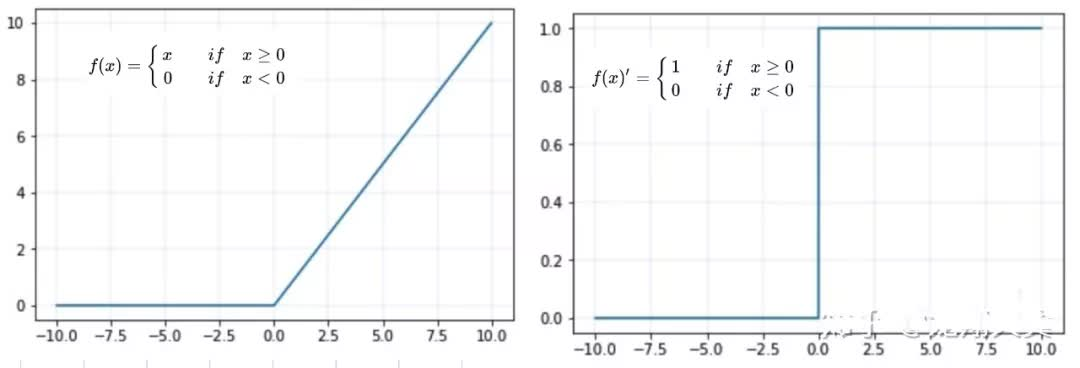
\includegraphics[width = 1\textwidth]{ReLU}
\caption{ReLU函数及其导数}
\label{piture:10}
\end{figure}

\section{正则化}

在机器学习中一切抑制过拟合现象的方法都可以被称作是正则化方法,例如集合学习,数据增强,dropout,修改损失函数等。这里我们主要介绍接下来工作中所用到的通过修改损失函数的正则化方法。

修改损失函数的正则化方法主要有L1正则化(见公式~\ref{eq:9}~),L2正则化(见公式~\ref{eq:10}~)和Smooth L1正则化(见公式~\ref{eq:11}~)。


\begin{align}
L_1(x) ={} & |x| \label{eq:9}\\
L_2(x) ={} & x^2 \label{eq:10}\\
smooth_{L_1}(x) ={} & \left\{
\begin{array}{rl}
\label{eq:11}
0.5x^2 & \text{if } |x| < 1\\
|x|-0.5 & \text{otherwise}
\end{array}\right.
\end{align}

其中$x$为预测值与真值之间的差异。

三个损失函数对$x$的导数分别为:

\begin{align}
\frac{\dif L_1(x)}{\dif x} ={} & \left\{
\begin{array}{rl}
\label{eq:12}
1 & \text{if } x \geqslant 0\\
-1 & \text{otherwise}
\end{array}\right.\\
\frac{\dif L_2(x)}{\dif x} ={} & 2x \label{eq:13}\\
\frac{\dif smooth_{L_1}(x)}{\dif x} ={} & \left\{
\begin{array}{rl}
\label{eq:14}
x & \text{if } |x| < 1\\
\pm 1 & \text{otherwise}
\end{array}\right.
\end{align}

根据公式~\ref{eq:12}~,$L_1$对$X$的导数是常数。这将带来一个问题,那就是训练后期时,真值和预测值之间的差值很小,但$L_1$对$X$的导数仍然不变,导致神经网络难以继续收敛。更致命的是,$L_1$在零点导数不唯一,会影响训练的收敛。

观察公式~\ref{eq:13}~,$L_1$对$X$的导数与$X$呈正相关。所以刚开始训练时真值和预测值之间的差值很大,导致损失函数的梯度也很大,会使得训练不稳定。同时离群点会占据loss的主要部分,造成训练的失败。

而Smooth L1 Loss(公式~\ref{eq:14}~)结合了L1 Loss以及L2 Loss的优点,它既可以较快地收敛,又能降低对离群点的敏感度,使得梯度变化较小,训练不易波动。

\section{本章小结}

本章主要介绍了卷积神经网络的一些信息,为后续研究BlazePose算法打好基础,重点阐述了CNN的组成部件,CNN的反向传播算法,以及激活函数的选择和一些常见的正则化方法。


% Local Variables:
% TeX-master: "../main"
% TeX-engine: xetex
% End:
